\documentclass[11pt]{article}
\usepackage[utf8]{inputenc}
\usepackage[T1]{fontenc}
%\usepackage{newtxtext,newtxmath}
\usepackage{amsmath}
\usepackage{multicol}
\usepackage{geometry}
\usepackage{tikz}
\usetikzlibrary{shapes.geometric, arrows.meta}
\usepackage{enumitem}
\usepackage{xcolor}
\usepackage{titlesec}

% Configurações de layout
\geometry{a4paper, left=1cm, right=1cm, top=0.5cm, bottom=1.2cm}
\setlength{\columnseprule}{0.4pt}
\setlength{\baselineskip}{1.0\baselineskip}

% Cores para títulos
\titleformat{\section}{\normalfont\Large\bfseries\color{blue}}{\thesection}{1em}{}
\titleformat{\subsection}{\normalfont\large\bfseries\color{red}}{\thesubsection}{1em}{}
\titleformat{\subsubsection}{\normalfont\normalsize\bfseries\color{black}}{\thesubsubsection}{1em}{}

\title{\textcolor{blue}{Medição e Cálculo: Perímetro, Área, Volume, Capacidade e Massa}}
\author{Professor: Jefferson}
\date{}

\begin{document}

\maketitle
\vspace{-1cm}

\begin{center}
\large{Nome: \underline{\hspace{8cm}} \quad Turma: \underline{\hspace{3cm}}}
\end{center}

\begin{multicols}{2}

\section*{1. Perímetro}
O perímetro é a soma dos lados de uma figura plana.

\subsection*{Fórmulas e Figuras}
\begin{itemize}
    \item \textbf{ Quadrado e Retângulo}:
    \[
    P = 2(a + b)
    \]
    \begin{center}
    \begin{tikzpicture}[scale=0.8]
        \draw (0,0) rectangle (3,2);
        \node at (1.5,0) [below] {$a$};
        \node at (0,1) [left] {$b$};
    \end{tikzpicture}
    \end{center}
    
    \item \textbf{Triângulo}:
    \[
    P = a + b + c
    \]
    \begin{center}
    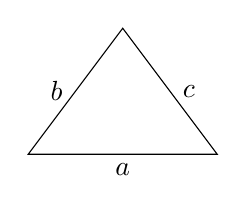
\begin{tikzpicture}[scale=0.8]
        \draw (0,0) -- (3,0) -- (1.5,2) -- cycle;
        \node at (1.5,0) [below] {$a$};
        \node at (0.7,1) [left] {$b$};
        \node at (2.3,1) [right] {$c$};
    \end{tikzpicture}
    \end{center}

\end{itemize}

\subsection*{Atividade}
Calcule o perímetro de:
\begin{enumerate}[label=\alph*)]
    \item  Calcule o perímetro de um quadrado com lado 5 cm.
    \textbf{Resposta:} $P = 4 \times 5 = 20$ cm
    
    \item  Um retângulo tem perímetro 30 cm. Se um lado mede 8 cm, qual o outro lado?
    \textbf{Resposta:} $30 = 2(8 + b) \Rightarrow 15 = 8 + b \Rightarrow b = 7$ cm
    
    \item  Um triângulo equilátero tem lado 6 cm. Qual seu perímetro?
    \textbf{Resposta:} $P = 3 \times 6 = 18$ cm
     
    \item  Um terreno retangular tem perímetro 60 m. Se a largura é metade do comprimento, quais são suas dimensões?
    \textbf{Resposta:} Seja $c$ o comprimento e $l = c/2$ a largura. \\
    $60 = 2(c + c/2) \Rightarrow 30 = 1.5c \Rightarrow c = 20$ m, $l = 10$ m
\end{enumerate}

\section*{2. Área}
Área é a medida da superfície (unidades: m², cm²).

\subsection*{Fórmulas e Figuras}
\begin{itemize}
    \item \textbf{Retângulo}:
    \[
    A = b \times h
    \]
    \begin{center}
    \begin{tikzpicture}[scale=0.7]
        \draw (0,0) rectangle (4,2);
        \node at (2,0) [below] {$b$};
        \node at (0,1) [left] {$h$};
    \end{tikzpicture}
    \end{center}
    
    \item \textbf{Triângulo}:
    \[
    A = \frac{b \times h}{2}
    \]
    \begin{center}
    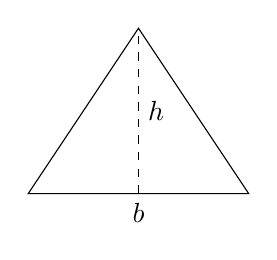
\begin{tikzpicture}[scale=0.7]
        \draw (0,0) -- (4,0) -- (2,3) -- cycle;
        \draw[dashed] (2,0) -- (2,3);
        \node at (2,0) [below] {$b$};
        \node at (2,1.5) [right] {$h$};
    \end{tikzpicture}
    \end{center}
    
    \item \textbf{Círculo}:
    \[
    A = \pi r^2
    \]
    \begin{center}
    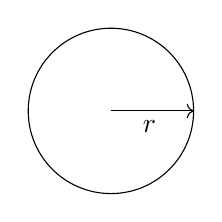
\begin{tikzpicture}[scale=0.7]
        \draw (0,0) circle (1.5);
        \draw[->] (0,0) -- (1.5,0);
        \node at (0.7,0) [below] {$r$};
    \end{tikzpicture}
    \end{center}

    \item \textbf{Cone}:
\[
A_{\text{total}} = \pi r (r + g)
\]
\begin{center}
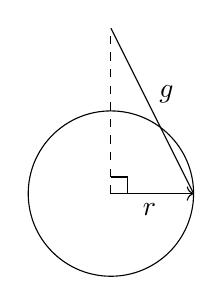
\begin{tikzpicture}[scale=0.7]
    % Base (círculo)
    \draw (0,0) circle (1.5);
    % Linha do raio (seta)
    \draw[->] (0,0) -- (1.5,0);
    \node at (0.7,0) [below] {$r$};
    % Geratriz (linha lateral)
    \draw[dashed] (0,0) -- (0,3);
    \draw (0,3) -- (1.5,0);
    \node at (0.7,1.8) [right] {$g$};
    % Ângulo reto
    \draw (0.3,0) -- (0.3,0.3) -- (0,0.3);
\end{tikzpicture}
\end{center}

\item \textbf{Trapézio}:

\[
A = \frac{(B + b) \times h}{2}
\]
\begin{center}
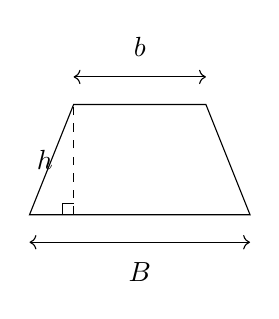
\begin{tikzpicture}[scale=0.7]
    % Trapézio (lados não paralelos inclinados)
    \draw (0,0) -- (4,0) -- (3.2,2) -- (0.8,2) -- cycle;
    
    % Base maior (B)
    \draw[<->] (0,-0.5) -- (4,-0.5);
    \node at (2,-0.7) [below] {$B$};
    
    % Base menor (b)
    \draw[<->] (0.8,2.5) -- (3.2,2.5);
    \node at (2,2.7) [above] {$b$};
    
    % Altura (h) - tracejada
    \draw[dashed] (0.8,0) -- (0.8,2);
    \node at (0.6,1) [left] {$h$};
    
    % Ângulo reto na altura
    \draw (0.6,0) -- (0.6,0.2) -- (0.8,0.2);
\end{tikzpicture}
\end{center}

\end{itemize}

\subsection*{Atividade}
Calcule a área de:
\begin{enumerate}[label=\alph*)]
    \item  Calcule a área de um retângulo com base 7 cm e altura 3 cm.
    \textbf{Resposta:} $A = 7 \times 3 = 21$ cm²
    
    \item  Um quadrado tem área 36 m². Qual seu lado?
    \textbf{Resposta:} $l = \sqrt{36} = 6$ m
    
    \item  Um triângulo tem base 12 cm e área 48 cm². Qual sua altura?
    \textbf{Resposta:} $48 = \frac{12 \times h}{2} \Rightarrow h = 8$ cm
    
    \item  Um círculo tem raio 5 m. Calcule sua área (use π = 3,14).
    \textbf{Resposta:} $A = 3.14 \times 5^2 = 78.5$ m²
    
    \item  Um terreno tem formato de trapézio com bases 10 m e 6 m e altura 4 m. Qual sua área?
    \textbf{Resposta:} $A = \frac{(10+6) \times 4}{2} = 32$ m²
\end{enumerate}

\section*{3. Volume}
Volume mede o espaço ocupado (unidades: m³, cm³).

\subsection*{Fórmulas e Figuras}
\begin{itemize}
    \item \textbf{Cubo}:
    \[
    V = a^3
    \]
    \begin{center}
    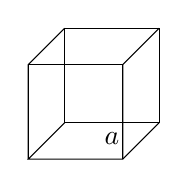
\begin{tikzpicture}[scale=0.6]
        \draw (0,0,0) -- (2,0,0) -- (2,2,0) -- (0,2,0) -- cycle;
        \draw (0,0,0) -- (0,0,2) -- (2,0,2) -- (2,0,0);
        \draw (2,0,2) -- (2,2,2) -- (2,2,0);
        \draw (0,2,0) -- (0,2,2) -- (0,0,2);
        \draw (0,2,2) -- (2,2,2);
        \node at (1,0,0) [below] {$a$};
    \end{tikzpicture}
    \end{center}
    
    \item \textbf{Cilindro}:
    \[
    V = \pi r^2 h
    \]
    \begin{center}
    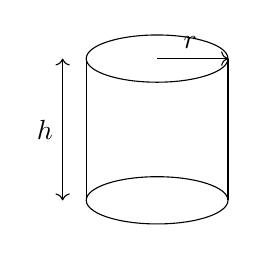
\begin{tikzpicture}[scale=0.6]
        \draw (0,0) ellipse (1.5 and 0.5);
        \draw (-1.5,0) -- (-1.5,-3);
        \draw (1.5,0) -- (1.5,-3);
        \draw (0,-3) ellipse (1.5 and 0.5);
        \draw[->] (0,0) -- (1.5,0);
        \node at (0.7,0) [above] {$r$};
        \draw[<->] (-2,0) -- (-2,-3);
        \node at (-2,-1.5) [left] {$h$};
    \end{tikzpicture}
    \end{center}
\end{itemize}

\begin{itemize}
    \item \textbf{Cone}:
    \[
    V = \frac{1}{3}\pi r^2 h
    \]
    \begin{center}
    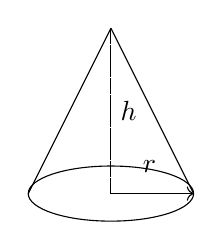
\begin{tikzpicture}[scale=0.7]
        % Base elíptica (vista em perspectiva)
        \draw (0,0) ellipse (1.5cm and 0.5cm);
        
        % Linhas laterais
        \draw (-1.5,0) -- (0,3);
        \draw (1.5,0) -- (0,3);
        
        % Linha da altura (tracejada)
        \draw[dashed] (0,0) -- (0,3);
        \node at (0,1.5) [right] {$h$};
        
        % Raio (seta)
        \draw[->] (0,0) -- (1.5,0);
        \node at (0.7,0.2) [above] {$r$};
        
        % Linha de contorno posterior (tracejada)
        \draw[dashed] (0,3) -- (0,0) -- (1.5,0);
    \end{tikzpicture}
    \end{center}
\end{itemize}

\subsection*{Atividade}
Calcule o volume de:
\begin{enumerate}[label=\alph*)]
    \item Calcule o volume de um cubo com aresta 4 m.
    \textbf{Resposta:} $V = 4^3 = 64$ m³
    
    \item Um paralelepípedo tem dimensões 3 cm × 4 cm × 5 cm. Qual seu volume?
    \textbf{Resposta:} $V = 3 \times 4 \times 5 = 60$ cm³
    
    \item Um cilindro tem raio 3 cm e altura 8 cm. Calcule seu volume (use π = 3,14).
    \textbf{Resposta:} $V = 3.14 \times 3^2 \times 8 = 226.08$ cm³
    
    \item Uma pirâmide tem base quadrada com lado 5 m e altura 9 m. Qual seu volume?
    \textbf{Resposta:} $V = \frac{1}{3} \times 5^2 \times 9 = 75$ m³
    
    \item Um cone tem raio 3 cm e altura 8 cm. Calcule seu volume (use π = 3,14).
    \textbf{Resposta:} $V = \frac{1}{3} \times 3.14 \times 3^2 \times 8 = 75.36$ cm³
\end{enumerate}

\section*{4. Capacidade}
Relação entre volume e litros: 

\begin{itemize}
    \item $1 \, \text{L} = 1 \, \text{dm}^3$
    \item $1 \, \text{m}^3 = 1000 \, \text{L}$
\end{itemize}

\subsection*{Exemplo}
Uma piscina tem $V = 8 \, \text{m}^3$. Quantos litros comporta?  
\[
8 \, \text{m}^3 = 8000 \, \text{L}
\]

\subsection*{Atividade}
Converta:
\begin{enumerate}[label=\alph*)]
    \item  Converta 2 m³ para litros.
    \textbf{Resposta:} $2 \times 1000 = 2000$ L
    
    \item  Quantos litros cabem em um recipiente com 4000 cm³?
    \textbf{Resposta:} $4000 \div 1000 = 4$ L (pois $1 \text{L} = 1000 \text{cm}^3$)
    
    \item  Uma piscina tem 8 m de comprimento, 5 m de largura e 1,2 m de profundidade. Quantos litros de água ela comporta?
    \textbf{Resposta:} $V = 8 \times 5 \times 1.2 = 48$ m³ $= 48,000$ L
    
    \item  Um tanque cilíndrico tem raio 0,5 m e altura 1,5 m. Qual sua capacidade em litros?
    \textbf{Resposta:} $V = \pi \times 0.5^2 \times 1.5 \approx 1.178$ m³ $= 1,178$ L
    
    \item  Uma caixa d'água cúbica tem capacidade de 27.000 L. Qual a medida de sua aresta?
    \textbf{Resposta:} $V = 27$ m³, $a = \sqrt[3]{27} = 3$ m
\end{enumerate}

\section*{5. Massa e Densidade}
\[
\text{Densidade} (d) = \frac{\text{Massa} (m)}{\text{Volume} (V)}
\]

\subsection*{Exemplo}
Um objeto tem $V = 20 \, \text{cm}^3$ e $d = 2.7 \, \text{g/cm}^3$. Qual sua massa?  
\[
m = d \times V = 2.7 \times 20 = 54 \, \text{g}
\]

\subsection*{Atividade}

\begin{enumerate}[label=\alph*)]
    \item  Um objeto tem V = 15 cm³ e m = 45 g. Qual sua densidade?
    \textbf{Resposta:} $d = \frac{45}{15} = 3$ g/cm³
    
    \item  Um líquido tem d = 0,9 g/cm³. Se V = 300 cm³, qual sua massa?
    \textbf{Resposta:} $m = 0.9 \times 300 = 270$ g
    
    \item  Um bloco de metal pesa 810 g e tem densidade 3 g/cm³. Qual seu volume?
    \textbf{Resposta:} $V = \frac{810}{3} = 270$ cm³
    
    \item  Uma esfera de prata (d = 10,5 g/cm³) tem raio 2 cm. Calcule sua massa.
    \textbf{Resposta:} $V = \frac{4}{3}\pi r^3 \approx 33.51$ cm³, $m = 10.5 \times 33.51 \approx 351.86$ g
    
    \item  Um cubo de ferro (d = 7,87 g/cm³) tem massa 1 kg. Qual a medida de sua aresta?
    \textbf{Resposta:} $V = \frac{1000}{7.87} \approx 127.06$ cm³, $a \approx \sqrt[3]{127.06} \approx 5.03$ cm
\end{enumerate}
\end{multicols}

\end{document}
